\section{Introduction}

In Bitcoin~\cite{bitcoin}, a valid block must satisfy the
\emph{proof-of-work} inequality $H(B) < T$, where
$H$ is a hash function and $T$ is a small \emph{target}.
Simply put, valid blocks must have hashes that begin with a desired number of $0$s.
Some blocks satisfy the inequality better than others:
They have a bunch of \emph{extra} zeroes at the front of their hash.
Nevertheless, these ``heavier'' blocks are counted all the same when choosing
which chain to mine on.
We posit that the weight of a block is information
that can be useful to improve the protocol.
In this paper, we introduce \emph{\poem}.
We modify the fork choice rule of Bitcoin to take this information into account,
achieving better confirmation latency.

\noindent
\myparagraph[Construction overview]
Miners still mine on the heaviest chain. We only change how chains are scored.
In Bitcoin, every block counts for the same work\footnote{Bitcoin blocks can count differently when
difficulty adjusts, but count the same during the same epoch. Our analysis is in the
static population setting~\cite{backbone}, where the population does not change with time.}.
In \poem, we give each block a score equal to the number of \emph{extra} zeroes at the front of its hash,
a value we call its \emph{intrinstic work}. Honest parties adopt the chain with the most total
intrinsic work.

% \iftwocolumn
% \begin{figure*}
%   \centering
%   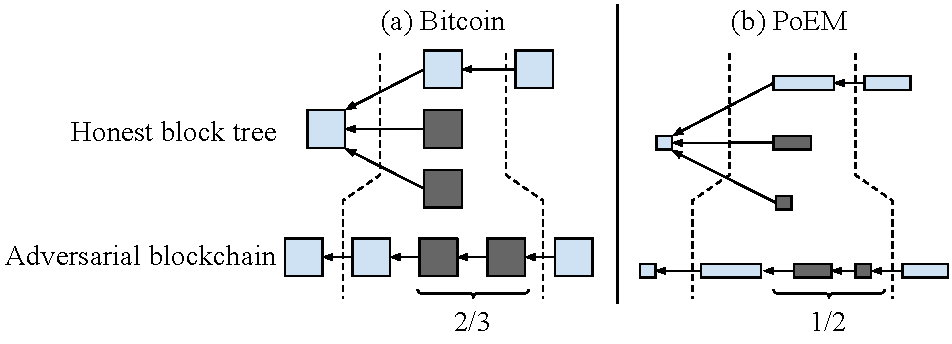
\includegraphics[width=0.6\textwidth,keepaspectratio]{figures/poem_work_wasted.pdf}
%   \caption{The same block mining successes awarded to the honest parties (top) or the adversary (bottom)
%            with equal mining power on Bitcoin (left) or PoEM (right) respectively. The adversary can place
%            all blocks in one sequence because she does not incur any network delay. The honest parties,
%            due to the delay, may place blocks at the same height (dashed section of duration $\Delta$).
%            In this example, when $3$ honest blocks were found almost simultaneously, $2$ out of
%            them were abandoned in Bitcoin and did not make it to the canonical longest chain
%            (top-most chain).
%            In the PoEM example, $2$ out of $3$ of the honest blocks were abandoned, but the cumulative intrinsic
%            work wasted only happened to be $1/2$ of the intrinsic work produced during this interval.
%            We illustrate the intrinsic work of a block by its size.}
%   \label{fig:poem-wasted-work}
% \end{figure*}
% \else
% \begin{figure*}
%   \centering
%   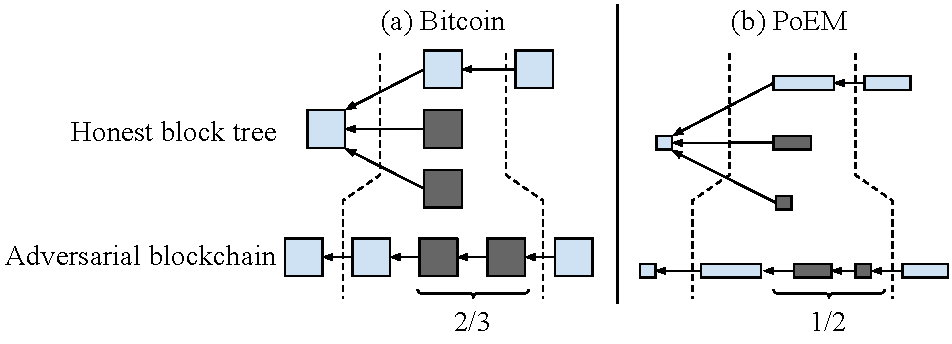
\includegraphics[width=0.8\textwidth,keepaspectratio]{figures/poem_work_wasted.pdf}
%   \caption{The same block mining successes awarded to the honest parties (top) or the adversary (bottom)
%            with equal mining power on Bitcoin (left) or PoEM (right) respectively. The adversary can place
%            all blocks in one sequence because she does not incur any network delay. The honest parties,
%            due to the delay, may place blocks at the same height (dashed section of duration $\Delta$).
%            In this example, when $3$ honest blocks were found almost simultaneously, $2$ out of
%            them (shaded) were abandoned in Bitcoin and did not make it to the canonical longest chain
%            (top-most chain).
%            In the PoEM example, $2$ out of $3$ of the honest blocks were abandoned, but the cumulative intrinsic
%            work wasted only happened to be $1/2$ of the intrinsic work produced during this interval.
%            In PoEM (right), we illustrate the intrinsic work of a block by its size.}
% \fi

\import{./}{figures/waste.tex}

To guarantee security, it suffices~\cite{eiar} that the work of any honest chain grows
faster than the work of the adversary's chain.
Suppose we have $n$ blocks produced in quick succession.
If they are honestly produced, they will be placed in parallel due to network delays,
forming $n$ forks.
If they are adversarially produced, since no network delay is incurred, they will be placed in series,
forming a chain of length $n$.
In Bitcoin, all blocks count the same constant amount of work $w$. So the honest chain grows by $w$,
and the adversarial chain grows by $n w$.
In PoEM, each block is scored differently: $w_1, w_2, \dots, w_n$, but has an expected work of $w$.
The adversarial chain grows by the sum of its blocks' work, $\sum_{i=1}^n w_i$.
In expectation, this is equal to $n w$, same as Bitcoin.
However, the honest chain now grows by the heaviest block's work: $\max_i w_i$,
which in expectation is greater than $w$. Hence, in expectation, honest PoEM chains grow
faster than honest Bitcoin chains in relation to the adversary's chain.

Let's look at the example in Figure~\ref{fig:poem-wasted-work}.
The same blocks, with the same amount of work, are given to both the adversary and the honest parties.
The adversary places all her blocks in series, while the honest blocks are necessarily placed in parallel
due to network delay.
In Bitcoin, the adversary makes $3$ times the progress that the honest parties make.
However, in PoEM, the adversary only makes $2$ times the progress that the honest parties make.
This means that honest work is more effectively utilized in PoEM than in Bitcoin.
Less honest work is wasted.

\noindent
\myparagraph[Our contributions]
\begin{itemize}
  \item We construct a protocol which retains the same level of security as Bitcoin, while achieving
        better confirmation latency because the block production rate can be safely increased.

  \item We simulate over $3{,}000$ years of continuous-time executions of both Bitcoin and PoEM
        using a combination of numeric and analytic techniques across a range of parameters
        and conclude that PoEM is $40\%$ faster in latency than Bitcoin for a $10\%$ adversary.

  \item We prove the security of PoEM in the Bitcoin Backbone~\cite{backbone} model. This
        requires novel techniques such as the
        \emph{real-valued random oracle}, a hash model that returns a \emph{continuous} value.
        We prove it behaves identically to the usual random oracle with overwhelming probability.

  \item We deployed a production testnet in which
        more than $2{,}000$ miners from the community participated
        with an average hash rate of $50$ GH/s using ProgPoW~\cite{progpow}.
\end{itemize}

\noindent
\myparagraph[Related work]
Bitcoin was first proven secure in the static population setting~\cite{backbone},
and later also studied in the variable population setting~\cite{varbackbone}.
The idea of using a more nuanced proof-of-work inequality in which some blocks
are considered heavier than others was first put forth by Andrew Miller~\cite{highway},
with the first complete protocol to utilize it being
Proofs of Proof-of-Work~\cite{popow}. These were later refined multiple times
to account for non\-/interactivity~\cite{nipopows}, backwards compatibility~\cite{velvet-nipopows},
onlineness~\cite{logspace}, on-chain data efficiency~\cite{compact-superblocks},
gas consumption~\cite{gasefficient-nipopows},
bribing resilience~\cite{soft-power},
and variable populations~\cite{dionyziz}.
We are the first to modify the fork choice rule to take these refinements into
account, following \ifanonymous
the
\else
our
\fi
previous short report ``POEM: Proof of Entropy Minima''~\cite{poem-short},
where the entropic fork choice rule was defined but not analyzed.
Our work only changes the PoW inequality.
Other mechanisms refining the fork choice rule
are orthogonal and can be combined with our approach, yielding even
further performance gains.
Such examples include GHOST~\cite{ghost},
PHANTOM~\cite{phantom}, SPECTRE~\cite{spectre}, and GhostDAG~\cite{ghostdag}.
Additional mechanisms towards improving the latency and throughput
of proof-of-work blockchains at the consensus
layer, also composable with ours, include parallel chains~\cite{parallel-chains},
separation of transaction/consensus blocks~\cite{prism},
hybrid approaches between proof-of-work and proof-of-stake~\cite{byzcoin},
and the use of microblocks~\cite{bitcoin-ng}.